\documentclass[]{BasiliskReportMemo}
\usepackage{AVS}


\newcommand{\submiterInstitute}{Autonomous Vehicle Simulation (AVS) Laboratory,\\ University of Colorado}

\newcommand{\ModuleName}{test\textunderscore sunlineSuKF}
\newcommand{\subject}{Sunline Switch-uKF Module and Test}
\newcommand{\status}{Initial document}
\newcommand{\preparer}{T. Teil}
\newcommand{\summary}{This module implements and tests a Switch Unscented Kalman Filter in order to estimate the sunline direction.}


\begin{document}


\makeCover



%
%	enter the revision documentation here
%	to add more lines, copy the table entry and the \hline, and paste after the current entry.
%
\pagestyle{empty}
{\renewcommand{\arraystretch}{2}
\noindent
\begin{longtable}{|p{0.5in}|p{4.5in}|p{1.14in}|}
\hline
{\bfseries Rev}: & {\bfseries Change Description} & {\bfseries By} \\
\hline
Draft & Initial Revision & T. Teil \\
\hline

\end{longtable}
}

\newpage
\setcounter{page}{1}
\pagestyle{fancy}

\tableofcontents
~\\ \hrule ~\\

%\begin{figure}[htb]
%	\centerline{
%	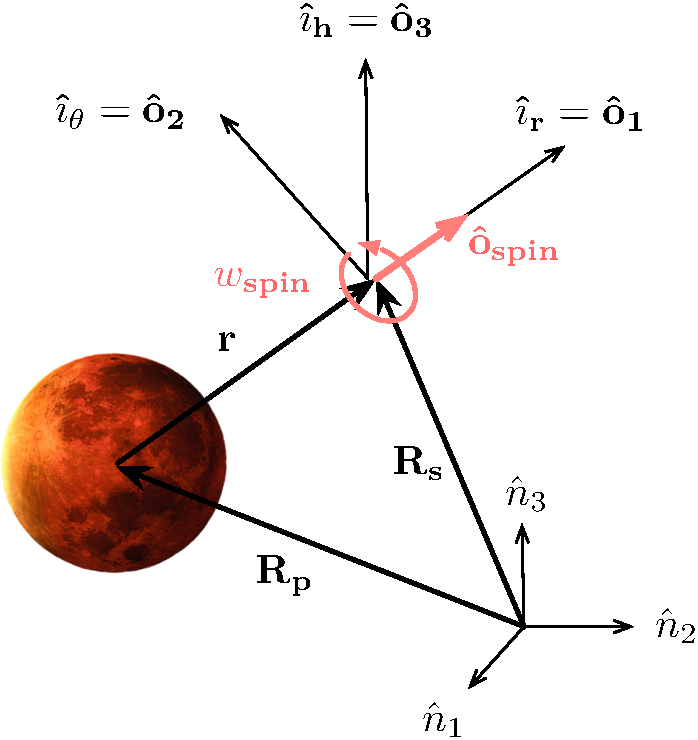
\includegraphics[]{Figures/Fig1}
%	}
%	\caption{Sample Figure Inclusion.}
%	\label{fig:Fig1}
%\end{figure}

\section{Introduction}
The Switch Unscented Kalman filter (SuKF) in the AVS Basilisk simulation is a sequential
filter implemented to give the best estimate of the desired states.
In this method we estimate the sun heading as well as the spacecraft rotation rate along the observable axes.
The SuKF reads in the message written by the coarse sun sensor, and writes a message 
containing the sun estimate. 

This document summarizes the content of the module, how to use it, and the test that 
was implemented for it. More information on the filter derivation can be found in Reference [\citenum{Teil:2018fe}], and more information on the square root unscented filter can be found in Reference [\citenum{Wan2001}] (attached alongside this document).

\section{Filter kinematics}

\subsection{Filter Derivation} %%%

The Switch-uKF attempts to avoid subtracting any terms from the state, while still removing the unobservable component of the rate. In order to do this, an appropriate frame must be defined.
In order to not track the rate component alongside the sunline direction, that vector needs to be one of the basis vectors of the frame. It is decided to be the first vector for the frame, and therefore in that frame, $\omega_1$ the component of the rotation rate can be removed from the states. 
This frame is called $\mathcal{S}_1 = \{\hat{\bm s}_1 = \frac{\bm d}{|\bm d|}, \hat{\bm s}_2, \hat{\bm s}_3 \}$. This is seen in Figure \ref{fig:Switches}, where the dotted line represents the $30 \dg$ threshold cone before switching frames. 

\begin{figure}[t]
	\centering
	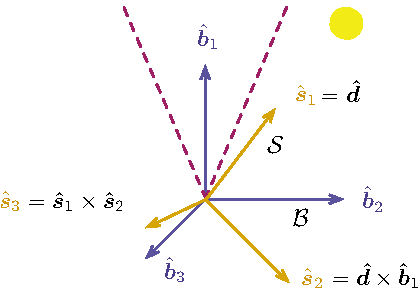
\includegraphics[]{./Figures/Switches}
	\caption{Frame built off the body frame for Switch filters}
	\label{fig:Switches}
\end{figure}

The second vector of the frame must be created using only $\bm d$, and the body frame vectors. The first intuitive decision, is to use $\hat{\bm b}_1$ of the body frame and define $\bm s_2$ in Equation \eqref{eq:s2}. The third vector $\hat{\bm s}_3$ of the $\mathcal{S}_1$ frame, is naturally created from the first two.
\begin{equation}\label{eq:s2}
\hat{\bm s}_2 = \frac{\hat{\bm s}_1 \times \hat{\bm b}_1}{|\hat{\bm s}_1 \times \hat{\bm b}_1|} \hspace{2cm} \hat{\bm s}_3 = \frac{\hat{\bm s}_1 \times \hat{\bm s}_2}{|\hat{\bm s}_1 \times \hat{\bm s}_2|}
\end{equation}
The problem that arises is the singularity that occurs when $\hat{\bm b}_1$ and $\bm d$ become aligned: this frame becomes undefined. In order to counteract this, using a similar process as the shadow set used for Modified Rodrigues Parameters [\citenum{schaub}], a second frame is created. This frame $\mathcal{S}_2 =  \{\hat{\bar{\bm s}}_1 = \hat{\bm s}_1, \hat{\bar{\bm s}}_2 , \hat{\bar{\bm s}}_3 \}$ is created with the same first vector, but constructs $\hat{ \bar{\bm s}}_2$ using $\hat{\bm b}_2$ of the body frame as in Equation \eqref{eq:s2bar}. The last vector, once again, finishes the orthonormal frame.
\begin{equation}\label{eq:s2bar}
\hat{\bar{\bm s}}_2 = \frac{\hat{\bar{\bm s}}_1 \times \hat{\bm b}_2}{|\hat{\bar{\bm s}}_1 \times \hat{\bm b}_2|}
\end{equation}
With both these frames, $\mathcal{S}_1$ and $\mathcal{S}_2$, the singularities can always be avoided. Indeed, $\mathcal{S}_1$ becomes singular when $\bm d$ approches $\hat{\bm b}_1$, while $\mathcal{S}_2$ becomes singular when the sunheading approaches $\hat{\bm b}_2$. By changing frames, whenever the sunline gets within a safe cone of $30 \dg$ (a modifiable value) of $\hat{\bm b}_1$, the frame is rotated into $\mathcal{S}_2$, which is not singular. Similarly, when $\bm d$ approches $\hat{\bm b}_2$ the frame is switched back to $\mathcal{S}_1$.

Because the two frames share the sunline vector $\bm d$, this vector is the same in both frames. This is a clear advantage as this is the vector we desire to estimate, and not having to rotate it avoids numerical issues.
The rotation of the rates is done by computing the following DCMs, of which all the vectors are known.
\begin{equation}\label{eq:DCMs}
 [\mathcal{B}\mathcal{S}_1] = \begin{bmatrix} \leftexp{B}{\hat{\bm s}_1} & \leftexp{B}{\hat{\bm s}_2} & \leftexp{B}{\hat{\bm s}_3}\end{bmatrix} \hspace{1cm}  [\mathcal{B}\mathcal{S}_2] = \begin{bmatrix} \leftexp{B}{\hat{\bar{\bm s}}_1} & \leftexp{B}{\hat{\bar{\bm s}}_2} & \leftexp{B}{\hat{\bar{\bm s}}_3}\end{bmatrix} \hspace{1cm}  [\mathcal{S}_2\mathcal{S}_1] = [\mathcal{B}\mathcal{S}_2] ^T [\mathcal{B}\mathcal{S}_1] 
\end{equation}

\subsection{Filter Dynamics} %%%

The filter is therefore derived with the states being $\bm X =\begin{bmatrix}\leftexp{B}{\bm d} & \omega_2 & \omega_3 \end{bmatrix}^{T}$, given that $\bm \omega_{\mathcal{S}/\mathcal{B}} = \leftexp{S}{\begin{bmatrix} \omega_1 & \omega_2 &\omega_3\end{bmatrix}}^T$. The rates of $\mathcal{S}$ relative to the body and inertial frame are related as such: $\bm \omega_{\mathcal{S}/\mathcal{N}} - \bm \omega_{\mathcal{S}/\mathcal{B}}  = \bm \omega_{\mathcal{B}/\mathcal{N}}$. Since $\omega_1$ is unknown, it is set to zero. Furthermore, since the sun heading is considered to be constant in the inertial frame over the period of time required for attitude determination and control, the equation becomes  $- \bar{\bm \omega}_{\mathcal{S}/\mathcal{B}}  = \bar{\bm \omega}_{\mathcal{B}/\mathcal{N}}$. 

${\bm \omega}_{\mathcal{S}/\mathcal{B}}$ is estimated directly by the filter, and its skew matrix can be computed by setting $\omega_1$ to zero (in the absence of information). This defines $\tilde{\bm \omega}_{\mathcal{B}/\mathcal{N}}$ as a function of known parameters. The dynamics are therefore given by Equations \eqref{eq:dynSwitch} and \eqref{eq:dynmatSwitch}, where $ \tilde{[\bm d]}(2,3)$ corresponds to the $2^{\text{nd}}$ and $3^{\text{rd}}$ columns of the $ \tilde{[\bm d]}$ matrix.
\begin{align}
\label{eq:dynSwitch}
\bm X' = \bm F(\bm X) &=  \begin{bmatrix}  \leftexp{B}{ \bm d'} \\  \omega_2' \\ \omega_3' \end{bmatrix} =   \begin{bmatrix}  -\leftexp{B}{\bar{\bm \omega}_{\mathcal{B}/\mathcal{N}}} \times \leftexp{B}{\bm d}\\ 0 \\ 0\end{bmatrix}  =   \begin{bmatrix} [\mathcal{B}\mathcal{S}]\leftexp{S}{\begin{bmatrix} 0 \\ \omega_2 \\ \omega_3\end{bmatrix}} \times \leftexp{B}{\bm d}\\ 0 \\ 0\end{bmatrix}  
\\\label{eq:dynmatSwitch}
[A]&= \begin{bmatrix} \frac{\partial \bm F (\bm d, t_i)}{\partial \bm X}  \end{bmatrix}  =   \begin{bmatrix} [ \leftexp{B}{\tilde{\bar{\bm \omega}}_{\mathcal{S}/\mathcal{B}}}] & - \tilde{[\bm d]}[\mathcal{B}\mathcal{S}](2,3) \\  [0]_{2\times 3} &  [0]_{2\times 2} \end{bmatrix} 
\end{align}
This formulation leads to simple dynamics, much simpler than those of the filter which subtracts the unobservable states, yet can actually estimate the observable of the rate, instead of using past estimates of $\bm d$. 

In regard to the SR-uKF version of this filter, the same coefficients are used: $\alpha = 0.02$, and $\beta = 2$. 


\subsection{Switching Frames} %%%

When switching occurs, the switch matrix $[W]$ can be computed in Equation \eqref{eq:switchMat} using the previously computed DCMs. This equation assumes the switch is going from frame 1 to frame 2 (the reciprocal is equivalent), and $[\mathcal{S}_2 \mathcal{S}_1](2,3)$ corresponds to the $2^{\text{nd}}$ and $3^{\text{rd}}$ columns of the $[\mathcal{S}_2 \mathcal{S}_1]$ matrix. 
\begin{equation}\label{eq:switchMat}
[W] = \begin{bmatrix} [I]_{3\times 3} & [0]_{3 \times 2} \\ [0]_{2 \times 3} & [\mathcal{S}_2 \mathcal{S}_1](2,3)\end{bmatrix}
\end{equation}
The new states $\bm X$ and covariance [P] after the switch are therefore given in Equation \eqref{eq:switchEq}
\begin{equation}\label{eq:switchEq}
\bar{\bm X} = [W] \bm X \hspace{2cm} [\bar{P}] = [W] [P] [W]^T
\end{equation}
When writing out the values of the state and covariance, it is necessary to bring it back into the body frame, using the $[\mathcal{B}\mathcal{S}]$ DCM ($\mathcal{S}$ representing the current frame in use).

\subsection{Measurements}
The measurement model is given in equation \ref{eq:meas}, and the $H$ matrix defined as $H = \left[\frac{\partial \bm G (\bm X, t_i)}{\partial \bm X}\right]^{*}$ is given in equation $\ref{eq:Hmat}$. 

In this filter, the only measurements used are from the coarse sun sensor. For the $i^\mathrm{th}$ sensor, the measurement is simply given by the dot product of the sunline heading and the normal to the sensor. This yields easy partial derivatives for the H matrix, which is a matrix formed of the rows of transposed normal vectors (only for those which received a measurement). Hence the $H$ matrix has a changing size depending on the amount of measurements. 

\begin{equation}\label{eq:meas}
\bm G_i(\bm X) = \bm n_i \cdot \bm d
\end{equation}

\begin{equation}\label{eq:Hmat}
\bm H(\bm X) = \begin{bmatrix} \bm n_1^T \\ \vdots \\ \bm n_i^T \end{bmatrix} 
\end{equation}


\section{Filter Set-up, initialization, and I/O}

\subsection{User initialization}

In order for the filter to run, the user must set a few parameters:

\begin{itemize}
\item The unscented filter has 3 parameters that need to be set, and are best as: \\
      \texttt{ filterObject.alpha = 0.02} \\
      \texttt{ filterObject.beta = 2.0} \\
      \texttt{ filterObject.kappa = 0.0} 
\item The angle threshold under which the coarse sun sensors do not read the measurement: \\ 
\texttt{FilterContainer.sensorUseThresh = 0.}
\item The process noise matrix: \\
   \texttt{qNoiseIn = numpy.identity(5)} \\
   \texttt{ qNoiseIn[0:3, 0:3] = qNoiseIn[0:3, 0:3]*0.01*0.01} \\
   \texttt{ qNoiseIn[3:5, 3:5] = qNoiseIn[3:5, 3:5]*0.001*0.001} \\
    \texttt{filterObject.qNoise = qNoiseIn.reshape(25).tolist()}
\item The measurement noise value, for instance: \\
 \texttt{FilterContainer.qObsVal = 0.001}
\item The initial covariance: \\
 \texttt{Filter.covar =} \\
  \texttt{ [1., 0.0, 0.0, 0.0, 0.0, \\
                          0.0, 1., 0.0, 0.0, 0.0,\\
                          0.0, 0.0, 1., 0.0, 0.0,\\
                          0.0, 0.0, 0.0, 0.02, 0.0,\\
                          0.0, 0.0, 0.0, 0.0, 0.02]}
 \item The initial state :\\
 \texttt{Filter.state =[0.0, 0.0, 1.0, 0.0, 0.0]}
\end{itemize}

The messages must also be set as such:

\begin{itemize}
\item    \texttt{ filterObject.navStateOutMsgName = "sunline$\_$state$\_$estimate"}
\item    \texttt{ filterObject.filtDataOutMsgName = "sunline$\_$filter$\_$data"}
\item   \texttt{ filterObject.cssDataInMsgName = "css$\_$sensors$\_$data"}
\item   \texttt{ filterObject.cssConfInMsgName = "css$\_$config$\_$data"}
\end{itemize}

\subsection{Inputs and Outputs}

The SuKF reads in the measurements from the coarse sun sensors. These are under the form of a list of cosine values. Knowing the normals to each of the sensors, we can therefore use them to estimate sun heading.


\section{Test Design}
The unit test for the sunlineSuKF module is located in:\\

\noindent
{\tt fswAlgorithms/attDetermination/sunlineSuKF/$\_$UnitTest/test$\_$SunlineSuKF.py} \\

As well as another python file containing plotting functions:

\noindent
{\tt fswAlgorithms/attDetermination/sunlineSuKF/$\_$UnitTest/SunlineSuKF$\_$test$\_$utilities.py} \\

The test is split up into 3 subtests. The first test creaks up all of the individual filter methods and tests them individually. These notably go over the square-root unscented filter specific functions. The second test verifies that in the case where the state is zeroed out from the start of the simulation, it remains at zero. The third test verifies the behavior of the time update with a measurement modification in the middle of the run. 

\subsection{Individual tests}

In each of these individual tests, random inputs are fed to the methods and their values are computed in parallel in python. These two values are then compared to assure that the correct computations are taking place. 
\begin{itemize}
\item \underline{QR Decomposition}: This tests the QR decomposition function which returns just the R matrix. Tolerance to absolute error $\epsilon = 10^{-15}$.

\textcolor{ForestGreen}{Passed}
\item \underline{LU Decomposition}: This tests the LU Decomposition accuracy. Tolerance to absolute error $\epsilon = 10^{-14}$.

\textcolor{ForestGreen}{Passed}
\item \underline{LU backsolve}: This tests the LU Back-Solve accuracy. Tolerance to absolute error $\epsilon = 10^{-14}$.

\textcolor{ForestGreen}{Passed}
\item \underline{LU matrix inverse}: This tests the LU Matrix Inverse accuracy. Tolerance to absolute error $\epsilon = 10^{-14}$.

\textcolor{ForestGreen}{Passed}
\item \underline{Cholesky decomposition}: This tests the Cholesky Matrix Decomposition accuracy. Tolerance to absolute error $\epsilon = 10^{-14}$.

\textcolor{ForestGreen}{Passed}
\item \underline{L matrix inverse}: This tests the L Matrix Inverse accuracy. Tolerance to absolute error $\epsilon = 10^{-14}$.

\textcolor{ForestGreen}{Passed}

\item \underline{U matrix inverse}: This tests the U Matrix Inverse accuracy. Tolerance to absolute error $\epsilon = 10^{-12}$.

\textcolor{ForestGreen}{Passed}
\end{itemize}

\subsection{Static Propagation}


\input{AutoTeX/StatesPlotprop.tex}

This test also takes no measurements in, and propagates with the expectation of no change. It then tests that the states and covariance are as expected throughout the time of simulation. Plotted results are seen in Figure \ref{fig:StatesPlotprop}. We indeed see that the state and covariance that evolve nominally and without bias .

Tolerance to absolute error: $\epsilon = 10^{-10}$

\subsection{Full Filter test}

This test the filter working from start to finish. No measurements are taken in for the first 20 time steps. Then a heading is given through the CSS message. Halfway through the simulation, measurements stop, and 20 time steps later a different heading is read. The filter must be robust and detect this change. This test is parametrized for different test lengths, different initial conditions, different measured headings, and with or without measurement noise. All these are successful.

\vspace{0.2cm}
Tolerance to absolute error without measurement noise: $\epsilon = 10^{-10}$

\textcolor{ForestGreen}{Passed}

Plotted results are seen in Figures \ref{fig:StatesPlotupdate}, and \ref{fig:PostFitupdate}. Figure \ref{fig:StatesPlotupdate} shows the state error and covariance over the run. We see the covariance initially grow, then come down quickly as measurements are used. It grows once again as the measurements stop before bringing the state error back to zero with a change in sun heading. 

Figure \ref{fig:PostFitupdate} shows the post fit residuals for the filter, with no measurement noise. We see that the observations are read in well an that the residuals are brought back down to zero.

\input{AutoTeX/StatesPlotupdate.tex}
\input{AutoTeX/PostFitupdate.tex}


\bibliographystyle{AAS_publication}   % Number the references.
\bibliography{references}   % Use references.bib to resolve the labels.



\end{document}
